\section{Evaluasi Sistem}
\subsection{\textit{Training}}
Proses training dilakukan sebanyak 1000 \textit{epochs} dan \textit{learning ra\-te} den\-gan nilai 0.005.
Nilai MSE yang didapatkan pada epoch ke 1000 ber\-ni\-lai \textbf{0.2385}, yang dapat dilihat pada gambar~\ref{fig:training}

\begin{figure}[H]
    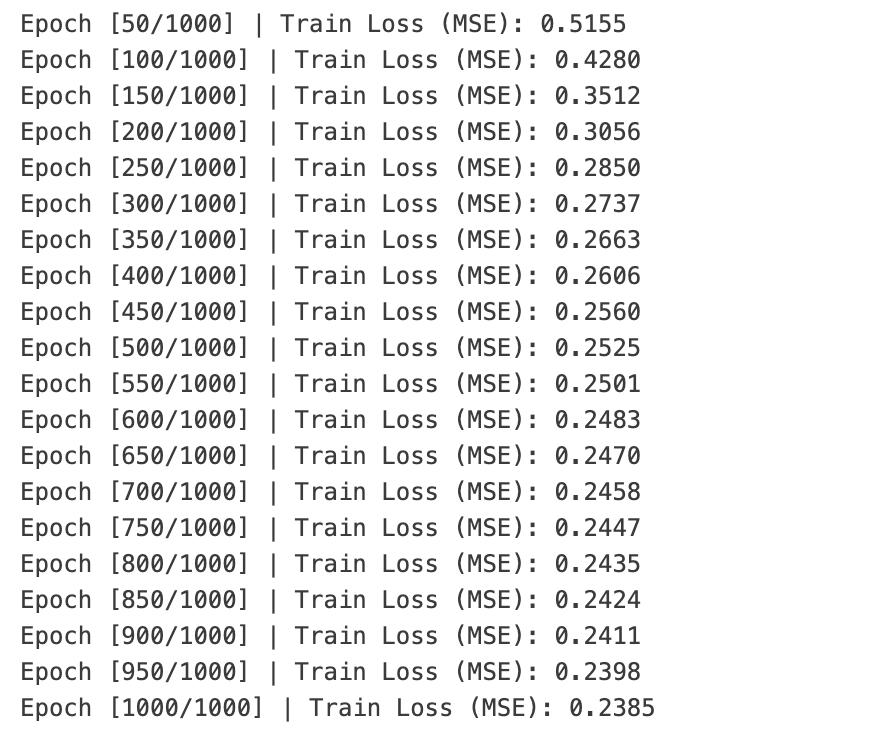
\includegraphics[width=0.8\textwidth]{training.png}
    \caption{Training}\label{fig:training}
\end{figure}
\subsection{Evaluasi}

Evaluasi model dilakukan dengan menggunakan MAE, RMSE\@ dan Koefisien Determinasi.
Hasil evaluasi adalah MAE sebesar \textbf{6.56 MPa}, RMSE sebesar \textbf{8.57 MPa} dan  Koefisien Determinasi sebesar \textbf{0.7165}.
